\chapter{Research Problem} \label{ch_research_problem}

The last chapter presented the state of the art in activity recognition, in general and within the perspective of robotics.
While the subject has been studied extensively in the recent years, the problem still provide a fertile research field to test different approaches.
Activity recognition is particularly relevant for autonomous robots.
It provides valuable knowledge from the environment necessary tu understand a situation, interact with people and learn from their actions. 

Also, ASP was presented as a methodology to treat problems of knowledge representation and reasoning.
Despite the main concepts of ASP were stated in the late 1980s, this approach of problem solving haven't been completely exploited, particularly in robotics, and still remains as a very active research area within the field of Logic Programming.

We are interested in exploring the possibilities of ASP in the context of autonomous robotics.
In general, as a tool to handle problems that require knowledge representation and reasoning, and in particular, related to the problem of activity recognition.

This chapter presents the main problem to be studied in this project: activity recognition with a mobile robot with an ASP-based approach.
It also introduces the structure of a framework to build a solution to the problem, putting special emphasis in the usage of ASP.
This framework can be built and integrated with current state of the art hardware and software tools. 
%The \textit{Library setting} (section \ref{sec_Library}) is used as a case to explain the ideas and as a potential environment for experimentation, necessary to set the path of future work.
%Finally, the approach is discussed to expose its strengths, its weaknesses, and the present expected outcome.


\section{Problem Description} \label{sec_problem}

% Description of the problem
The subject of study in this project is \textbf{ASP-based activity recognition with a mobile robot}.
The interest lies in the spatio-temporal relations that exist between activities and the environment, and how these can be obtained, handled and used by a mobile robot.

The problem of activity recognition is relevant for robots, particularly for those that share their environment with humans.
At the same time, ASP offers an interesting and novel approach for problems that require knowledge representation and reasoning.
These three parts: \textit{Activity Recognition} as a problem, \textit{Robotics} as a system platform, and \textit{ASP} as a set of techniques to treat problems that require knowledge representation and reasoning, they have been studied widely separately, but their integration still remains as an open field with particular challenges and potential solutions. 
This joint integration is the focus for this project.

ASP has not been fully exploited in robotic applications.
In a traditional logic programming approach for problem solving, a set of facts and rules is collected first to perform later an analysis \textit{a posteriori} (e.g. making questions).
But in robotics, new data is arriving continuously, and the knowledge that the robot has about the environment will need to be updated as soon as possible; some rules may not be valid any more, and also there is the need to handle unknown and uncertain statements.
Logic programming allows updates by adding and/or erasing premises and resetting the whole system, but in some ASP extensions this can be done online, e.g. ROSoClingo \ref{AndresOSSR13_rosoclingo}.

The target application is to be able to build a system, on top of a robot, that can be able to observe actively and annotate the ongoing activities in a location (e.g. a library). 
By using a robot, human perception is partially emulated, however, this will drive to situations with incomplete information, because most of the times, the robot won't be able to sense all the environment. 
It is an hypothesis for this project that the lack of sensory information can be complemented with a stronger cognitive approach, in this case, by considering domain knowledge.

The results of the system (recognized activities) can be used in different ways, but particularly as semantic knowledge, which has a meaning, a context and can be used for reasoning.
In this particular problem, activities have a spatial and temporal significance, that is the reason why they can be stored in a semantic map.
This, can eventually be useful for a robot to have a qualitative description of the environment, to augment its navigation capabilities and task planning, and also, to bridge the gap in human-robot interaction \citep{Kostavelis2015_SemMapSurv}.

%Going back to the library setting described in section \ref{sec_Library}. %TODO %TODO Add example


\section{Methodology} \label{sec_methodology}

This section presents the proposed approach to tackle the problem.

First, the target platform is an autonomous mobile robot.
In a general fashion, a control system for a robot can be simplified as a perception-action loop. %TODO %TODO Add image Perception-Action
An activity recognition system fits in by providing interesting features from the environment (activities) that a robot can use to improve its performance.

The figure \ref{fig:structure} presents the structure of the overall system.
The principal input are observations from the environment in the form of recognized features, e.g. humans, objects, etc.
Observations of the world are needed, in order to have a starting point to process.
Additionally to this, symbolic information will also be used in the form of a semantic map, domain knowledge (e.g. ontologies), previous experiences and finally, the activity representations.
The output of the system is a set of activities and features found on the environment, within a degree of confidence.

\begin{figure}[h]
\centering
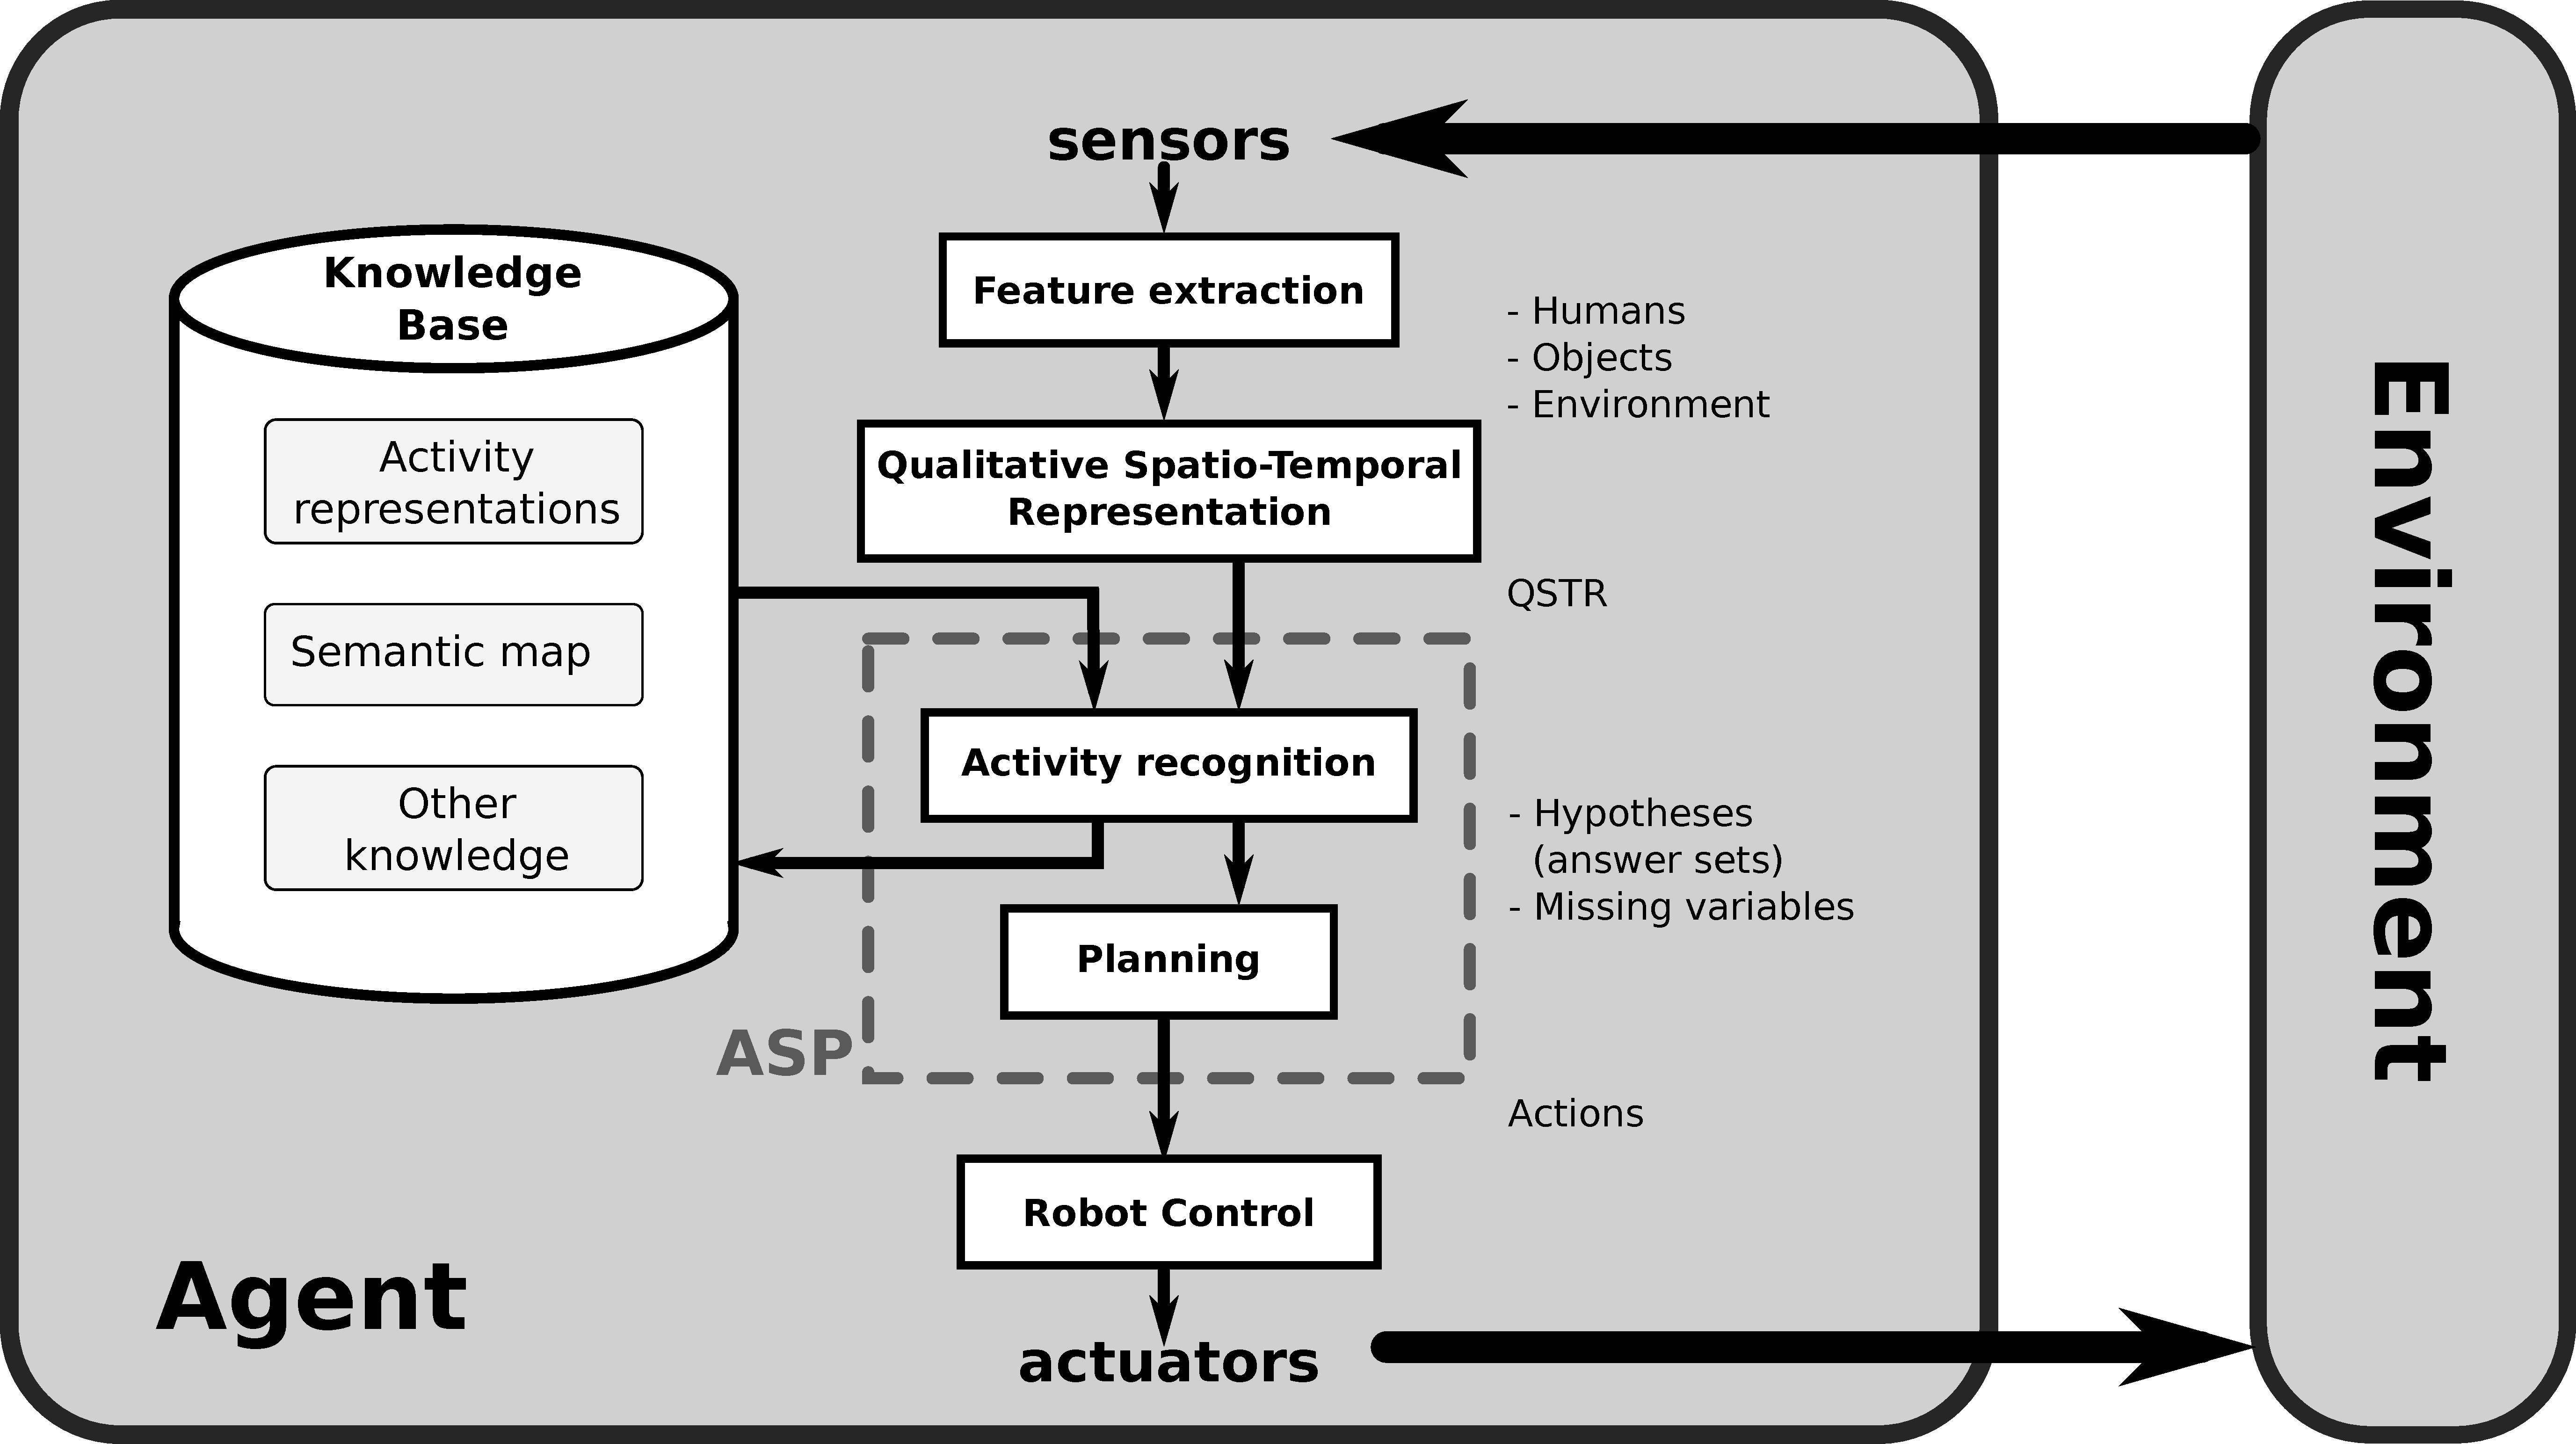
\includegraphics[width=\textwidth]{fig/img_structure.pdf}
\caption{Model for the ASP-based activity recognition system with a robot.}
\label{fig:structure}
\end{figure}


\subsection{Sensing and feature extraction}

The end target for this project are autonomous mobile robots, with this in mind, all the sensing is in charge of the robot. 
No building sensing (e.g. CCTV) or portable devices (e.g. cellphone, laptop) are allowed, this is the goal.
We are looking forward to use state-of-the-art sensing techniques, however, completely reliable sensing is not assured and improving sensing algorithms is beyond the scope of this project, the use of simulations and environment marks is considered for experimental purposes. 
%TODO Add "see next section/chapter" 

The features to be sensed will depend on the type of activities to be recognized.
By using the categorization of activities mentioned in section \ref{sec_problem}, we are interested in the mid-level activities.
This considers single human activities and interactions with other humans and/or objects, and excludes gestures and group activities.
So, human and object sensing are needed.
In the same fashion, the aim is to provide a robot with some understanding of activities within a spatio-temporal conceptualization by building a semantic map, so location and mapping are also a requirement, i.e. environment sensing.

All these give us a path to decompose the scene in three different categories within a 3D space \ref{fig:decomposition}: 
\begin{description}
\item[humans] detection, recognition, kinematic description, etc.
\item[objects] detection, recognition, kinematic description, etc.
\item[environment] localization, grid and topological maps, etc.
\end{description}

\begin{figure}[h]
\centering
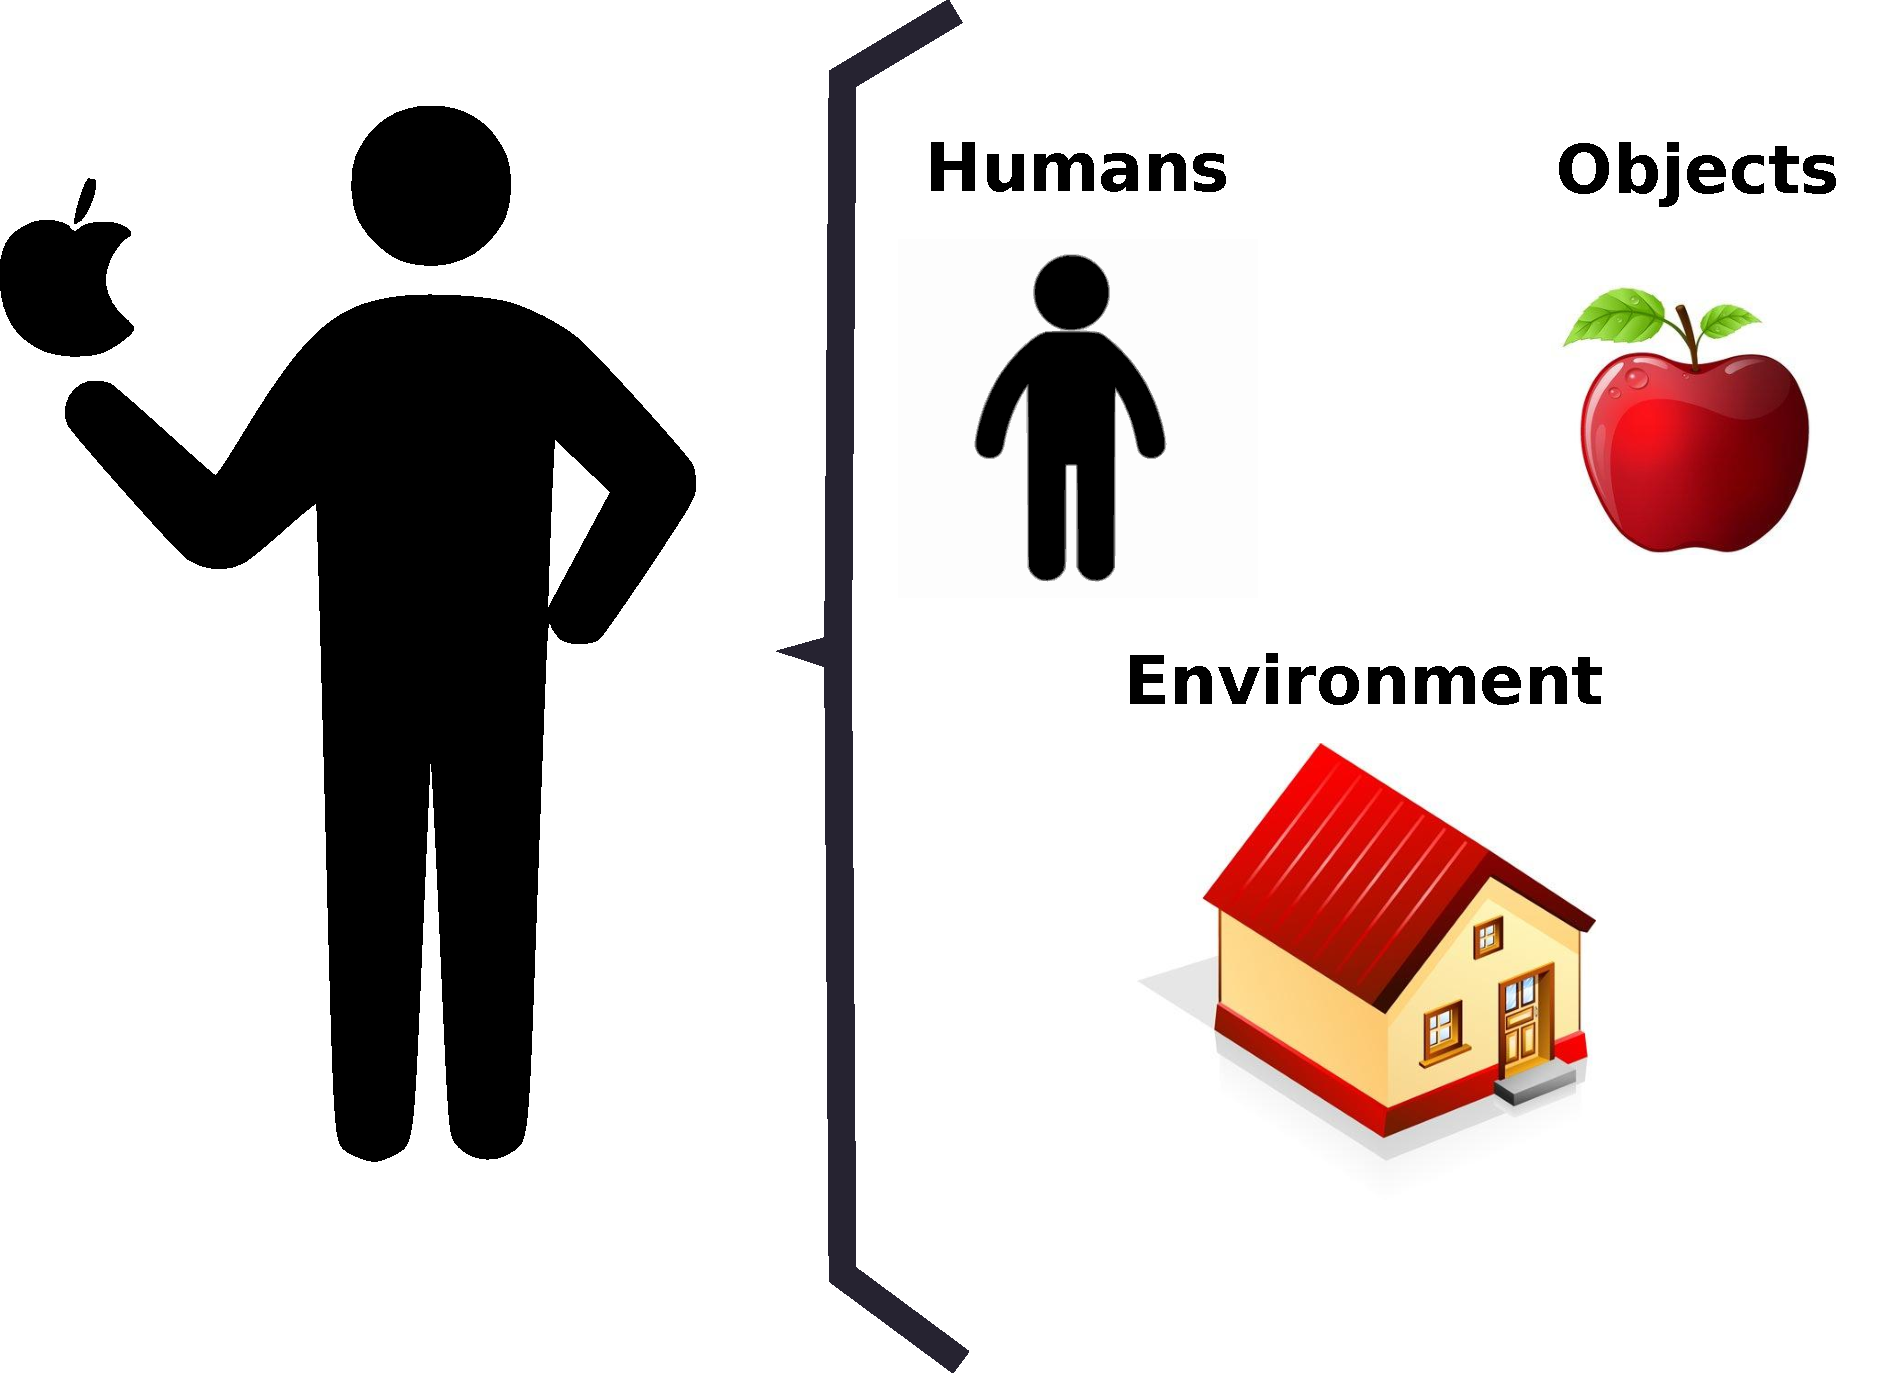
\includegraphics[width=3in]{fig/scene_dec.pdf}
\caption{Sensing will be targeting relevant features from humans, objects and from the environment.}
\label{fig:decomposition}
\end{figure}

%TODO  Add Image reference and image of scene decomposition.

\subsection{Qualitative Spatio-Temporal Representations}
QSTR were introduced briefly mentioned in chapter \ref{ch_relatedwork}.
They provide formal models to represent and reason about geometrical entities in space and time.
Space is handled with Qualitative Spatial Relations. %TODO Expand explanation and reference.
Time is usually modelled in events using Allen's interval algebra \ref{Allen83_MaintainingKnowledgeTemporal}. %TODO expand

A qualitative approach is desired as it proofs to be more robust to dynamic and non-deterministic environments.
It also avoids to depend on training data or parameters which are specific to a particular location, and drives the data towards a symbolic representation.
Finally, because it is a more human-alike approach, desired for a better human-robot interaction.

The idea here is to convert quantitative observations to qualitative, by representing the spatio-temporal relations between objects and/or persons, and eventually, with the environment too (e.g. regions of interests).

While it could be a temptation to build all possible relations between the entities of interest in a scene, this has proved to be an non-efficient approach \citep{Sridhar10_UnsupervisedLearning}, mostly because the combinatorial explosion of the amount  of possible relations. The relations to be handled have to be chosen in a more \textit{intelligent} fashion.

%TODO Add example.

\subsection{Knowledge Base}
Additionally to the observations, a knowledge is required, which contains symbolic information that will be used to process the 
observations.
First, and most importantly, the description of activities are required.
This also will include a description from the environment (i.e. a semantic map) and other domain knowledge that can potentially be used to infer new knowledge.

An important question here is about the origin of this knowledge, and in particular of the activities.
The simplest approach is to define the activity representations manually.
For some specific activities this can be enough, however, in general other strategies are required.
Activities can be learnt, from a human demonstrator or by analysing data from repeated situations.
Finally the representation of activities can be consulted in larger knowledge databases using some existing tools, e.g. wikiHow \citep{web_WikiHow}, OpenCyc \citep{web_OpenCyc}, KnowRob \citep{Tenorth09_Knowrob}, RoboEarth \citep{Zweigle2009_RoboEarth}.
Here the focus is to share knowledge between robotic system instead of learning it every time as this will take considerable computational effort.


%\subsection{Maintaining observations}

%The qualitative observations need to be maintained, because new observations will arrive along time, and some of them will need to be updated.
%For example, the qualitative representation of a person approaching to the entrance door may take many samples until the person is seen %crossing the door frame, and all these \textit{person-approaching-door} observations need to be merged into a single event and only the temporal relations between events may require to be updated.
%TODO Add example "Walking person to".


\subsection{Inferring activities}

At this point, the system has a set of qualitative observations in time and space of interesting features.
Along time, these observations should be updated or thrown to have a compact set of valid premises.

Now, the problem is to map the observations into an activity representation. 
As mentioned before, ASP provides a the techniques to solve difficult combinatorial problems. and in particular, search problem as satisfiability problems (SAT).
This is how, the observations become a set of constraints to find definitions (of activities) that satisfy them.

It should be noticed that the observations do not necessarily fulfil all the required parameters in the definition.
However, here is where ASP shows its usability by being able to provide candidate solutions, even when there are unknown parameters.

At the end we have a solution, or many possible solutions to the problem of correspondence between the observations and the defined activities.

%TODO Expand and include the example.


\subsection{Discriminate activities}

If there is unique correspondence, then this can be taken as solution for the problem\footnote{Nevertheless, it should the noted that, even though the ASP premises have a logical meaning, it will be very difficult to guarantee complete certainty.}. 
However, it is expected that this will barely be the case.
But, there are many possibilities available to find a solution.

First, additional knowledge sources can be considered.
These are, a semantic map of the environment and domain knowledge, which can be represented in ASP.

Secondly, a learning strategy can be implemented to find patterns of \textit{frequently occurring activities} in particular locations, by specific persons or with related objects. 
This is, to maintain a knowledge base of experiences.

Finally, the described system can take advantage of the fact that the robot is active.
The robot can interact with the environment and with persons, and it can choose points of interest in the scene.

For example, a robot may be watching a person in the library with an unknown object in the hands. 
The robot can create a belief, by context and by experience, that the object is a book.
However, he can also go closer to that person to have a better look of the object.
Finally, interaction is also possible, and the robot can simply ask the person which object is he/she holding.

One important observation should be made in the previous example, and this is, the fact that the robot should figure where to look, or what information is missing to improve its conclusions. 
This is an advantage, but also a necessity as it is very unlikely that a robot can have complete coverage of a scene.
In the example, the required knowledge is the identification of the object, which can be helpful to discriminate between to activities, e.g. eating and studying. 
Knowing which parts of the missing knowledge will help to improve the conclusions, or which ones are more important, gives a path to plan an active strategy for the robot to fulfil those perception holes.


\subsection{Robot Action}

Up to this point, the robot has created an internal model of a scene, regarding activities.
This model should be used, and could be incomplete.
The forward step is to close the loop and use activeness of the robot to improve the process of activity recognition. This can be done by implementing a plan that takes in consideration priorities as looking for missing information, surface coverage of a location, amount of collected information, points of interest, etc.



% Alternatives for each part
% > Observations
% > Knowledge (where? & how?, I'll do it by hand, but it's important to mention alternatives).
% > Representations
% *** CHECK THE orgnanization from the surveys
%   - Modelling activities in space (QSR)
%   - Modelling activities in time  (QSTR ~ Allen's, Fluent, Event, etc).
%   - Modelling activities semantically (Ontologies + Hierarchies)
% > Inference

% Test example

